\begin{savequote}[45mm]
\ascii{Do the simplest thing that could possibly work.}
\qauthor{\ascii{- Kent Beck}}
\end{savequote}

\chapter{物理设计} 
\label{ch:physical-design}

\section{头文件}

\begin{content}

\begin{regulation}
自定义头文件必须具有扩展名,以区分\cpp{}标准库的头文件;在团队内部,头文件、源文件扩展名类型必须保持一致性
\end{regulation}

表\reftbl{file-extension}列出了头文件和实现文件常见的扩展名,团队应该选择一类扩展名并保持团队内一致性。

\begin{table}[H]
\resizebox{0.95\textwidth}{!} {
\begin{tabular*}{1.2\textwidth}{@{}ll@{}}
\toprule
\ascii{文件类型} & \ascii{支持的扩展名} \\
\midrule
\ascii{头文件}  & \ascii{.h, .hpp, .hxx, .hh, h++, .tcc} \\
\ascii{源文件} & \ascii{.c, .C, .cpp, .cxx, .cc, .c++} \\ 
\bottomrule
\end{tabular*}
}
\caption{扩展名}
\label{tbl:file-extension}
\end{table}

\begin{regulation}
每一个头文件都应该具有独一无二的保护宏,并保持命名规则的一致性
\end{regulation}

命名规则包括两种风格:
\begin{enum}
  \eitem{\tt{INCL\_<PROJECT>\_<MODULE>\_<FILE>\_H}}
  \eitem{\ascii{全局唯一的随机序列码\footnote{例如\ascii{Eclipse}可以配置头文件的代码模板,\ascii{Visual
  C++}也存在类似的插件,其他\ascii{IDE}也存在类似的功能}}}
\end{enum}

第一种命名规则问题在于:当文件名重命名或移动目录时,需要同步修改头文件保护宏;推荐使用\ascii{IDE}随机自动地生成头文件保护宏,其更加快捷、简单、安全、有效\footnote{为了简化举例,后文的头文件定义,都略去了头文件宏保护符。}。

正例:
\begin{leftbar}
\begin{c++}
#ifndef INCL_CPPUNIT_AUTO_REGISTER_SUITE_H
#define INCL_CPPUNIT_AUTO_REGISTER_SUITE_H

#endif
\end{c++}
\end{leftbar}

或使用IDE随机自动生成

\begin{leftbar}
\begin{c++}
#ifndef INCL_ADCM_LLL_3465_DCPOE_ACLDDDE_479_YTEY_H
#define INCL_ADCM_LLL_3465_DCPOE_ACLDDDE_479_YTEY_H

#endif
\end{c++}
\end{leftbar}

反例:
\begin{leftbar}
\begin{c++}
// 因名称太短,存在名字冲突的可能性
#ifndef ACTION_H
#define ACTION_H

#endif
\end{c++}
\end{leftbar}

\begin{regulation}
路径名一律使用小写、下划线或中划线风格的名称;文件名应该与程序主要实体名称相同,可以使用驼峰命名,也可以使用小写、下划线或中划线分割的名字;实现文件的名字必须和头文件保持一致;更重要的是,团队内必须保持一致的命名风格
\end{regulation}

正例:
\begin{leftbar}
\begin{c++}
#include "html-parser/core/Attribute.h"
#include "yaml_parser.h"
\end{c++}
\end{leftbar}

反例:
\begin{leftbar}
\begin{c++}
// 路径名htmlParser使用了驼峰命名风格
#include "htmlParser/core/Attribute.h"
\end{c++}
\end{leftbar}

\begin{regulation}
包含头文件时,必须保持路径名、文件名大小写敏感
\end{regulation}

因为在\ascii{Windows},其大小写不敏感,编译时检查失效,代码失去了可移植性,所以在包含头文件时必须保持文件名的大小写敏感。

假如存在两个物理文件名分别为\ascii{SynchronizedObject.h, yaml\_parser.h}的文件。

正例:
\begin{leftbar}
\begin{c++}
#include "cppunit/core/SynchronizedObject.h"
#include "yaml_parser.h"
\end{c++}
\end{leftbar}

反例:
\begin{leftbar}
\begin{c++}
// 路径名、文件名大小写与真实物理路径、物理文件名称不符
#include "CppUnit/Core/SynchronizedObject.h"
#include "YAML_Parser.h"
\end{c++}
\end{leftbar}

\begin{regulation}
包含头文件时,路径分隔符一律使用\ascii{Unix}风格,拒绝使用\ascii{Windows}风格;即采用\code{/}
而不是使用\textbackslash{}分割路径
\end{regulation}

正例:
\begin{leftbar}
\begin{c++}
// 使用了Unix风格的路径分割符
#include "cppunit/core/SynchronizedObject.h"
\end{c++}
\end{leftbar}

反例:
\begin{leftbar}
\begin{c++}
// 使用了Windows风格的路径分割符
#include "cppunit\core\SynchronizedObject.h"
\end{c++}
\end{leftbar}

\begin{regulation}
使用\ascii{extern} \texttt{"}\ascii{C}\texttt{"}时,不要包括\ascii{include}语句
\end{regulation}

正例:
\begin{leftbar}
\begin{c++}
#include "oss_common.h"

#ifdef  __cplusplus
extern "C" {
#endif

void* OSS_alloc(size_t);
void  OSS_free(void*);

#ifdef  __cplusplus
}
#endif
\end{c++}
\end{leftbar}

反例:
\begin{leftbar}
\begin{c++}
#ifdef  __cplusplus
extern "C" {
#endif

// 错误地将include放在了extern "C"中
#include "oss_common.h"

void* oss_alloc(size_t);
void  oss_free(void*);

#ifdef  __cplusplus
}
#endif
\end{c++}
\end{leftbar}

\begin{regulation}
当以\clang{}提供实现时,头文件中必须使用\ascii{extern}
\texttt{"}\ascii{C}\texttt{"}声明,以便支持\cpp{}的扩展
\end{regulation}

正例:
\begin{leftbar}
\begin{c++}
#include "oss_common.h"

#ifdef  __cplusplus
extern "C" {
#endif

void* oss_alloc(size_t);
void  oss_free(void*);

#ifdef  __cplusplus
}
#endif
\end{c++}
\end{leftbar}

反例:
\begin{leftbar}
\begin{c++}
#include "oss_common.h"

void* oss_alloc(size_t);
void  oss_free(void*);
\end{c++}
\end{leftbar}

\begin{advise}
拒绝创建巨型头文件,将所有实体声明都放到头文件中
\end{advise}

不要把所有的宏、\ascii{const}常量、函数声明、类定义都要放在头文件中,而仅仅将外部依赖的实体声明放到头文件中。

实现文件也是一种信息隐藏的惯用技术,如果一些程序的实体不对外所依赖,则放在自己的实现文件中,一则可降低依赖关系,二则实现更好的信息隐藏。

巨型头文件必然造成了巨大的编译时依赖,不仅仅带来巨大的编译时开销,更重要的是这样的设计将太多的实现细节暴露给用户,导致后续版本兼容性的问题,阻碍了头文件进一步演进、修改、扩展的可能性,从而失去了软件的可扩展性。

不要认为提供一个大而全的头文件会给你的用户带来方便,用户因此而更加困扰。你应该更多地追求头文件的自满足性,而不是让你的用户还要关心头文件之间的依赖关系。

\end{content}

\section{物理设计原则}

\begin{content}

物理设计是\clang{}\ascii{/}\cpp{}语言中特有的一部分,遵循\reftbl{design-priciples-of-phy-design}中所列的设计原则,必然可以得到更加清晰、更加漂亮的头文件设计。

\begin{table}[H]
\resizebox{0.95\textwidth}{!} {
\begin{tabular*}{1.2\textwidth}{@{}ll@{}}
\toprule
\ascii{原则} & \ascii{基本含义} \\
\midrule
\ascii{自满足原则}  & \ascii{头文件本身是可以编译通过的} \\
\ascii{单一职责原则} & \ascii{头文件包含的实体的职责是单一的} \\ 
\ascii{最小依赖原则} & \ascii{绝不包含不必要的头文件} \\
\ascii{最小可见性原则} & \ascii{尽量封装隐藏类的成员} \\
\bottomrule
\end{tabular*}
}
\caption{物理设计四原则}
\label{design-priciples-of-phy-design}
\end{table}


\begin{principle}
自满足原则
\end{principle}

所有头文件都应该自满足的。所谓头文件自满足,即头文件自身是可编译成功的。

看一个具体的示例代码,这里定义了一个\ascii{TestCase.h}头文件。

反例:
\begin{leftbar}
\begin{c++}
struct TestCase : TestLeaf, TestFixture
{
    TestCase(const std::string &name="");
    
private:
    OVERRIDE(void run(TestResult *result));
    OVERRIDE(std::string getName() const);

private:
    ABSTRACT(void runTest());
    
private:
    const std::string name;
};
\end{c++}
\end{leftbar}

\ascii{TestCase}对父类\ascii{TestLeaf,
TestFixture}都存在编译时依赖,为了满足自满足原则,其自身必须包含其所有父类的头文件。

正例:
\begin{leftbar}
\begin{c++}
#include "cppunit/core/TestLeaf.h"
#include "cppunit/core/TestFixture.h"

struct TestCase : TestLeaf, TestFixture
{
    TestCase(const std::string &name="");
    
private:
    OVERRIDE(void run(TestResult &result));
    OVERRIDE(std::string getName() const);

private:
    ABSTRACT(void runTest());
    
private:
    const std::string name;
};
\end{c++}
\end{leftbar}

即使\ascii{TestCase}直接持有\ascii{name}的成员变量,但没有必要包含\ascii{std::string}的头文件,因为\ascii{TestCase}覆写了其父类的\ascii{getName}成员函数,父类为了保证自满足原则,自然已经包含了\ascii{std::string}的头文件。

同样的原因,也没有必要在此前置声明\ascii{TestResult},因为父类可定已经声明过了。

\begin{regulation}
实现文件的第一行代码必然是包含其对应的头文件
\end{regulation}

创建对应的实现文件\ascii{TestCase.cpp},并将自身头文件的进行包含,并置在实现文件的第一行,这是验证头文件自满足的最好的办法。

正例:
\begin{leftbar}
\begin{c++}
#include "cppunit/core/TestCase.h"
#include "cppunit/core/TestResult.h"
#include "cppunit/core/Functor.h"

namespace
{
    struct TestCaseMethodFunctor : Functor
    {
        typedef void (TestCase::*Method)();
    
        TestCaseMethodFunctor(TestCase &target, Method method)
           : target(target), method(method)
        {}
    
        bool operator()() const
        {
            target.*method();
            return true;
        }
    
    private:
        TestCase &target;
        Method method;
    };
}

void TestCase::run(TestResult &result)
{
    result.startTest(*this);
  
    if (result.protect(TestCaseMethodFunctor(*this, &TestCase::setUp))
    {
        result.protect(TestCaseMethodFunctor(*this, &TestCase::runTest)); 
    }

    result.protect(TestCaseMethodFunctor(*this, &TestCase::tearDown));

    result.endTest(*this);
}

...

\end{c++}
\end{leftbar}

反例:
\begin{leftbar}
\begin{c++}
#include "cppunit/core/TestResult.h"
#include "cppunit/core/Functor.h"
// 错误:没有放在第一行,无法校验其自满足性
#include "cppunit/core/TestCase.h"

namespace
{
    struct TestCaseMethodFunctor : Functor
    {
        typedef void (TestCase::*Method)();
    
        TestCaseMethodFunctor(TestCase &target, Method method)
           : target(target), method(method)
        {}
    
        bool operator()() const
        {
            target.*method();
            return true;
        }
    
    private:
        TestCase &target;
        Method method;
    };
}

void TestCase::run(TestResult &result)
{
    result.startTest(*this);
  
    if (result.protect(TestCaseMethodFunctor(*this, &TestCase::setUp)))
    {
        result.protect(TestCaseMethodFunctor(*this, &TestCase::runTest)); 
    }

    result.protect(TestCaseMethodFunctor(*this, &TestCase::tearDown));

    result.endTest(*this);
}

...

\end{c++}
\end{leftbar}

\begin{principle}
单一职责
\end{principle}

这是\ascii{SRP(Single Reponsibility
Priciple)}在头文件设计时的一个具体运用。头文件如果包含了其它不相关的元素,则包含该头文件的所有实现文件都将被这些不相关的元素所污染,重编译将成为一件高概率的事件。

如示例代码,将\ascii{OutputStream, InputStream}同时定义在一个头文件中,将违背该原则。
本来只需只读接口,无意中被只写接口所污染。

反例:
\begin{leftbar}
\begin{c++}

#include "base/Role.h"

DEFINE_ROLE(OutputStream)
{
    ABSTRACT(void write());
};

DEFINE_ROLE(InputStream)
{
    ABSTRACT(void read());
};

#endif
\end{c++}
\end{leftbar}

正例:先创建一个\ascii{OutputStream.h}文件:
\begin{leftbar}
\begin{c++}
#include "base/Role.h"

DEFINE_ROLE(OutputStream)
{
    ABSTRACT(void write());
};
\end{c++}
\end{leftbar}

再创建一个\ascii{InputStream.h}文件:

\begin{leftbar}
\begin{c++}
#include "base/Role.h"

DEFINE_ROLE(InputStream)
{
    ABSTRACT(void read());
};

\end{c++}
\end{leftbar}

\begin{principle}
最小依赖
\end{principle}

一个头文件只应该包含必要的实体,尤其在头文件中仅仅对实体的声明产生依赖,那么前置声明是一种有效的降低编译时依赖的技术。

反例:
\begin{leftbar}
\begin{c++}
#include <base/Role.h>
#include <cppunit/core/TestResult.h>
#include <string>

DEFINE_ROLE(Test)
{
    ABSTRACT(void run(TestResult& result));
    ABSTRACT(int countTestCases() const);
    ABSTRACT(int getChildTestCount() const);
    ABSTRACT(std::string getName() const);
};
\end{c++}
\end{leftbar}

如示例代码,定义了一个\ascii{xUnit}框架中的\ascii{Test}顶级接口,其对\ascii{TestResult}的依赖仅仅是一个声明依赖,并没有必要包含\ascii{TestResult.h},前置声明是解开这类编译依赖的钥匙。

值得注意的是,对标准库\ascii{std::string}的依赖,即使它仅作为返回值,但因为它实际上是一个\ascii{typedef},所以必须老实地包含其对应的头文件。事实上,如果产生了对标准库名称的依赖,基本上都需要包含对应的头文件。

另外,对\ascii{DEFINE\_ROLE}宏定义的依赖则需要包含相应的头文件,以便实现该头文件的自满足。

但是,\ascii{TestResult}仅作为成员函数的参数出现在头文件中,所以对\ascii{TestResult}的依赖只需前置声明即可。

正例:
\begin{leftbar}
\begin{c++}
#include <base/Role.h>
#include <string>

struct TestResult;

DEFINE_ROLE(Test)
{
    ABSTRACT(void run(TestResult& result));
    ABSTRACT(int countTestCases() const);
    ABSTRACT(int getChildTestCount() const);
    ABSTRACT(std::string getName() const);
};
\end{c++}
\end{leftbar}

在选择包含头文件还是前置声明时,很多程序员感到迷茫。其实规则很简单,在如下场景前置声明即可,无需包含头文件:

\begin{enum}
  \eitem{\ascii{指针}}
  \eitem{\ascii{引用}}
  \eitem{\ascii{返回值}}
  \eitem{\ascii{函数参数}}
\end{enum}

相反地,如果编译器需要知道实体的真正内容时,则必须包含头文件,此依赖也常常称为强编译时依赖。强编译时依赖主要包括如下几种场景:
\begin{enum}
  \eitem{\ascii{typedef}定义的实体\footnote{其实是弱编译时依赖,但为了避免代码重复,所以一般选择直接包含\ascii{typedef}的头文件}}
  \eitem{\ascii{继承}}
  \eitem{\ascii{宏}}
  \eitem{\ascii{inline}}
  \eitem{\ascii{template}}
  \eitem{\ascii{引用类内部成员时}}
  \eitem{执行\ascii{sizeof}运算}  
\end{enum}

\begin{principle}
最小可见性
\end{principle}

在头文件中定义一个类时,清晰、准确的\ascii{public, protected,
private}是传递设计意图的指示灯。其中\ascii{private}做为一种实现细节被隐藏起来,为适应未来不明确的变化提供便利的措施。

不要将所有的实体都\ascii{public},这无疑是一种自杀式做法。应该以一种相反的习惯性思维,尽最大可能性将所有实体\ascii{private},直到你被迫不得不这么做为止,依次放开可见性的权限。

如下例代码所示,按照\ascii{public-private,
function-data}依次排列类的成员,并对具有相同特征的成员归类,将大大改善类的整体布局,给读者留下清晰的设计意图。

\begin{leftbar}
\begin{c++}
#include "trans-dsl/action/Action.h"
#include "trans-dsl/utils/EventHandlerRegistry.h"

struct SimpleAsyncAction: Action
{
    template<typename T>
    Status waitOn(const EventId eventId, T* thisPointer,
             Status (T::*handler)(const TransactionInfo&, const Event&), 
             bool forever = false)
    {
        return registry.addHandler(eventId, thisPointer, handler, forever);
    }

    Status waitUntouchEvent(const EventId eventId);

private:
    OVERRIDE(Status handleEvent(const TransactionInfo&, const Event&));
    OVERRIDE(void kill(const TransactionInfo&, const Status)); 

private:
    DEFAULT(void, doKill(const TransactionInfo&, const Status));

private:
    EventHandlerRegistry registry;
};
\end{c++}
\end{leftbar}

\begin{regulation}
所有\ascii{override}的函数必然是\ascii{private}的,以保证按接口编程的良好设计原则
\end{regulation}

反例:
\begin{leftbar}
\begin{c++}
#include "html-parser/filter/NodeFilter.h"
#include <list>

struct AndFilter : NodeFilter
{
     void add(NodeFilter*);

     // 错误:本应该private
     OVERRIDE(bool accept(const Node&) const);

private:
     std::list<NodeFilter*> filters;
};
\end{c++}
\end{leftbar}

正例:
\begin{leftbar}
\begin{c++}
#include "html-parser/filter/NodeFilter.h"
#include <list>

struct AndFilter : NodeFilter
{
     void add(NodeFilter*);

private:
     OVERRIDE(bool accept(const Node&) const);

private:
     std::list<NodeFilter*> filters;
};
\end{c++}
\end{leftbar}

\end{content}

\section{Inline}

\begin{content}

\begin{regulation}
头文件中避免定义\ascii{inline}函数,除非\ascii{profiling}报告指出此函数是性能的关键瓶颈
\end{regulation}

\cpp{}语言将声明和实现进行分离,程序员为此不得不在头文件和实现文件中重复地对函数进行声明。这是一件痛苦的事情,驱使部分程序员直接将函数实现为\ascii{inline}。

但\ascii{inline}函数的代码作为一种不稳定的内部实现细节,被放置在头文件里,
其变更所导致的大面积的重新编译是个大概率事件,为改善微乎其微的函数调用性能与其相比将得不偿失。除非有相关\ascii{profiling}的测试报告,表明这部分关键的热点代码需要被放回头文件中。

让我们就像容忍头文件中宏保护符那样,也慢慢习惯\clang{}/\cpp{}天生给我们带来的这点点重复吧。

但需要注意,有两类特殊的情况,可以将实现\ascii{inline}在头文件中,因为为它们创建实现文件过于累赘和麻烦。

\begin{enum}
  \eitem{\ascii{virtual析构函数}}
  \eitem{\ascii{空的virtual函数实现}}
  \eitem{\ascii{\cpp{}11的default函数}}  
\end{enum}

\begin{regulation}
实现文件中鼓励\ascii{inline}函数实现
\end{regulation}

对于在编译单元内部定义的类而言,因为它的客户数量是确定的,就是它本身。另外,由于它本来就定义在源代码文件中,因此并没有增加任何“物理耦合”。所以,对于这样的类,我们大可以将其所有函数都实现为\ascii{inline}的,就像写\ascii{Java}代码那样,\ascii{Once
\& Only Once}。

以单态类的一种实现技术为例,讲解编译时依赖的解耦与匿名命名空间的使用。(首先,应该抵制单态设计的诱惑,单态其本质是面向对象技术中全局变量的替代品。滥用单态模式,犹如滥用全局变量,是一种典型的设计坏味道。只有确定在系统中唯一存在的概念,才能使用单态模式)。

实现单态,需要对系统中唯一存在的概念进行封装;但这个概念往往具有巨大的数据结构,如果将其声明在头文件中,无疑造成很大的编译时依赖。

反例:
\begin{leftbar}
\begin{c++}
#include "base/Status.h"
#include "base/BaseTypes.h"
#include "transport/ne/NetworkElement.h"
#include <vector>

struct NetworkElementRepository
{
    static NetworkElement& getInstance();

    Status add(const U16 id);
    Status release(const U16 id);
    Status modify(const U16 id);
    
private:
    typedef std::vector<NetworkElement> NetworkElements;
    NetworkElements elements;
};
\end{c++}
\end{leftbar}

受文章篇幅的所限,\ascii{NetworkElement.h}未列出所有代码实现,但我们知道\ascii{NetworkElement}拥有巨大的数据结构,上述设计导致所有包含\ascii{NetworkElementRepository}的头文件都被\ascii{NetworkElement}所间接污染。

此时,其中可以将依赖置入到实现文件中,解除揭开其严重的编译时依赖。更重要的是,它更好地遵守了按接口编程的原则,改善了软件的扩展性。

正例:
\begin{leftbar}
\begin{c++}
#include "base/Status.h"
#include "base/BaseTypes.h"
#include "base/Role.h"

DEFINE_ROLE(NetworkElementRepository)
{
    static NetworkElementRepository& getInstance();

    ABSTRACT(Status add(const U16 id));
    ABSTRACT(Status release(const U16 id));
    ABSTRACT(Status modify(const U16 id));
};
\end{c++}
\end{leftbar}

其实现文件包含\ascii{NetworkElement.h},将对其的依赖控制在本编译单元内部。

\begin{leftbar}
\begin{c++}
#include "transport/ne/NetworkElementRepository.h"
#include "transport/ne/NetworkElement.h"
#include <vector>

namespace
{
    struct NetworkElementRepositoryImpl : NetworkElementRepository
    {
        OVERRIDE(Status add(const U16 id))
        {
            // inline implements
        }

        OVERRIDE(Status release(const U16 id))
        {
            // inline implements
        }

        OVERRIDE(Status modify(const U16 id))
        {
            // inline implements
        }
    
    private:
        typedef std::vector<NetworkElement> NetworkElements;
        NetworkElements elements;
    };
}

NetworkElementRepository& NetworkElementRepository::getInstance()
{
    static NetworkElementRepositoryImpl inst;
    return inst;
}
\end{c++}
\end{leftbar}

此处,对\ascii{NetworkElementRepositoryImpl}类的依赖是非常明确的,仅本编译单元内,所有可以直接进行\ascii{inline},从而简化了很多实现\footnote{为了简化实现和举例,使用了\ascii{STL}中的\ascii{std::vector}。}。

\begin{regulation}
实现文件中提倡使用匿名\ascii{namespace}, 以避免命名冲突。
\end{regulation}

匿名\ascii{namespace}的存在常常被人遗忘,但它的确是一个利器。匿名\ascii{namespace}的存在,使得所有受限于编译单元内的实体拥有了明确的处所。

自此之后,所有\clang{}风格,并局限于编译单元内的\ascii{static}函数和变量;以及类似\ascii{Java}中常见的\ascii{private
static}的提取函数将常常被匿名\ascii{namespace}替代。

请记住匿名命名空间也是一种重要的信息隐藏技术。

\end{content}

\section{struct VS. class}

\begin{content}

\begin{advise}
在类定义时,建议统一使用\ascii{struct};但绝不允许混用\ascii{struct, class}。
\end{advise}

除了名字不同之外,\ascii{class}和\ascii{struct}唯一的差别是:默认可见性。这体现在定义和继承时。\ascii{struct}在定义一个成员,或者继承时,如果不指明,则默认为\ascii{public},而\ascii{class}则默认为\ascii{private}。

但这些都不是重点,重点在于定义接口和继承时,冗余\ascii{public}修饰符总让人不舒服。简单设计四原则告诉告诉我们,所有冗余的代码都应该被剔除。

但很多人会认为\ascii{struct}是\clang{}遗留问题,应该避免使用。但这不是问题,我们不应该否认在写\cpp{}程序时,依然在使用着很多\clang{}语言遗留的特性。关键在于,我们使用的是\clang{}语言中能给设计带来好处的特性,何乐而不为呢?

正例:
\begin{leftbar}
\begin{c++}
struct SelfDescribing
{
    virtual void describeTo(Description& description) const = 0;
    virtual ~SelfDescribing() {}
};
\end{c++}
\end{leftbar}

反例:
\begin{leftbar}
\begin{c++}
class SelfDescribing
{
public:
    virtual void describeTo(Description& description) const = 0;
    virtual ~SelfDescribing() {}
};
\end{c++}
\end{leftbar}

更重要的是,我们确信“抽象”和“信息隐藏”对于软件的重要性,这促使我将\ascii{public}接口总置于类的最前面成为我们的首选,\ascii{class}的特性正好与我们的期望背道而驰\footnote{\ascii{class}的特性正好适合于将数据结构捧为神物的程序员,它们常常将数据结构置于类声明的最前面。}

不管你信仰那一个流派,切忌不能混合使用\ascii{class}和\ascii{struct}。在大量使用前导声明的情况下,一旦一个使用\ascii{struct}的类改为\ascii{class},所有的前置声明都需要修改。

\begin{regulation}
定义\clang{}风格的结构体时,摒弃\ascii{struct tag}的命名风格。
\end{regulation}

\ascii{struct tag}彻底抑制了结构体前置声明的可能性,从而阻碍了编译优化的空间。

反例:
\begin{leftbar}
\begin{c++}
typedef struct tag_Cell
{
    WORD16 wCellId;
    WORD32 dwDlArfcn;
} T_Cell;

typedef struct
{
    WORD16 wCellId;
    WORD32 dwDlArfcn;
} T_Cell;
\end{c++}
\end{leftbar}

为了兼容\clang{}\footnote{在\clang{}语言中,如果没有使用\ascii{typedef},则定义一个结构体的指针,必须显式地加上\ascii{struct}关键字:\ascii{struct
T\_Cell *pcell},而\cpp{}没有这方面的要求。},并为结构体前置声明提供便利,如下解法是最合适的。

正例:
\begin{leftbar}
\begin{c++}
typedef struct T_Cell
{
    WORD16 wCellId;
    WORD32 dwDlArfcn;
} T_Cell;
\end{c++}
\end{leftbar}

\begin{advise}
如果性能不是关键问题,考虑使用\ascii{PIMPL}降低编译时依赖
\end{advise}

反例:
\begin{leftbar}
\begin{c++}
#include "JmpOnlyApiHook.h"

struct ApiHook
{
    ApiHook(const void* api, const void* stub)
      : stubHook(api, stub)
    {}

private:
    JmpOnlyApiHook stubHook;
};
\end{c++}
\end{leftbar}

正例:
\begin{leftbar}
\begin{c++}
struct ApiHookImpl;

struct ApiHook
{
    ApiHook(const void* api, const void* stub);
    ~ApiHook();

private:
    ApiHookImpl* This;
};
\end{c++}
\end{leftbar}

\begin{leftbar}
\begin{c++}
#include "ApiHook.h"
#include "JmpOnlyApiHook.h"

struct ApiHookImpl
{
   ApiHookImpl(const void* api, const void* stub)
     : stubHook(api, stub)
   {
   }

   JmpOnlyApiHook stubHook;
};

ApiHook::ApiHook( const void* api, const void* stub)
  : This(new ApiHookImpl(api, stub))
{
}

ApiHook::~ApiHook()
{
    delete This;
}
\end{c++}
\end{leftbar}

通过\ascii{ApiHookImpl*
This}的桥接,在头文件中解除了对\ascii{JmpOnlyApiHook}的依赖,将其依赖控制在本编译单元内部。

\end{content}

\section{template}

\begin{content}

\begin{advise}
当选择模板实现时,请最大限度地降低编译时依赖。
\end{advise}

当选择模板时,不得不将其实现定义在头文件中。当编译时依赖开销非常大时,编译模板将成为一种负担。设法降低编译时依赖,不仅仅为了缩短编译时间,更重要的是为了得到一个低耦合的实现。

反例:
\begin{leftbar}
\begin{c++}
#include "pub_typedef.h"
#include "pub_oss.h"
#include "oss_comm.h"
#include "pub_commdef.h"
#include "base/Assertions.h"
#include "base/Status.h"

struct OssSender
{
    OssSender(const PID& pid, const U8 commType)
      : pid(pid), commType(commType)
    {
    }
    
    template <typename MSG>
    Status send(const U16 eventId, const MSG& msg)
    {
        DCM_ASSERT_TRUE(OSS_SendAsynMsg(eventId, &msg, sizeof(msg), commType,(PID*)&pid) == OSS_SUCCESS); 
        return DCM_SUCCESS;
    }

private:
    PID pid;
    U8 commType;
};
\end{c++}
\end{leftbar}

为了实现模板函数\ascii{send},将\ascii{OSS}的一些实现细节暴露到了头文件中,包含\ascii{OssSender.h}的所有文件将无意识地产生了对\ascii{OSS}头文件的依赖。

提取一个私有的\ascii{send}函数,并将对\ascii{OSS}的依赖移入到\ascii{OssSender.cpp}中,对\ascii{PID}依赖通过前置声明解除,最终实现如代码所示。

正例:
\begin{leftbar}
\begin{c++}
#include "base/Status.h"
#include "base/BaseTypes.h"

struct PID;

struct OssSender
{
    OssSender(const PID& pid, const U16 commType)
      : pid(pid), commType(commType) 
    {
    }
    
    template <typename MSG>
    Status send(const U16 eventId, const MSG& msg)
    {
        return send(eventId, (const void*)&msg, sizeof(MSG));    
    }

private:
    Status send(const U16 eventId, const void* msg, size_t size);

private:
    PID pid;
    U8 commType;
};
\end{c++}
\end{leftbar}

识别哪些与泛型相关,哪些与泛型无关的知识,并解开此类编译时依赖是\cpp{}程序员的必备之技。

\begin{advise}
适时选择\ascii{Explicit Template Instantiated},降低模板的编译时依赖。
\end{advise}

模板的编译时依赖存在两个基本模型:包含模型,\ascii{export}模型。\ascii{export}模型受编译技术实现的挑战,最终被\cpp{}\ascii{11}标准放弃。

此时,似乎我们只能选择包含模型。其实,存在一种特殊的场景,是能做到降低模板编译时依赖的。

反例:
\begin{leftbar}
\begin{c++}
// RrmAdmitAction.h
#include "fw/action/SyncAction.h"
#include "dcm_inst/UeInstanceHelper.h"
#include "cell/UeCellObject.h"
#include "base/Assertions.h"

template <typename ADMIT_ROLE>
struct RrmAdmitAction : SyncAction
{
    OVERRIDE(Status exec(const TransactionInfo&))
    {
        ADMIT_ROLE* role = getCurrentCell(trans);
        DCM_ASSERT_VALID_PTR(role);

        return role->admit(); 
    }
}
\end{c++}
\end{leftbar}

\begin{leftbar}
\begin{c++}
// DrbSetupAdmitAction.h 
#include "rrm/actions/RrmAdmitAction.h"

struct DrbSetupAdmitAction : RrmAdmitAction<RrmDrbSetupRole> {};
\end{c++}
\end{leftbar}

如上的设计,泛型类\ascii{RrmAdmitAction}存在严重的编译时依赖,从而间接地污染了其他的文件。如果我们仔细分析,是有办法解开没有必要的编译时依赖的。

\begin{figure}
  \centering
  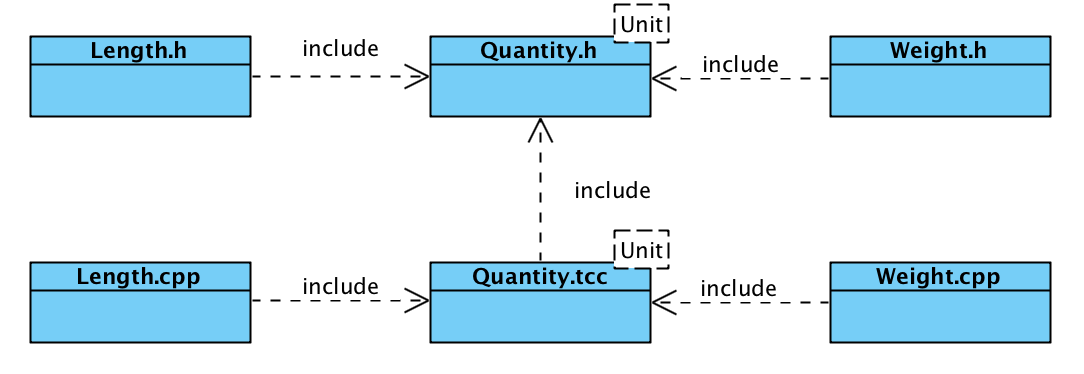
\includegraphics[width=0.8\textwidth]{figures/explict-template-inst}
  \caption{Explicit Template Instantiated}
  \label{fig:explict-template-inst}
\end{figure}

如\refig{explict-template-inst}所示,\ascii{DrbSetupAdmitAction.h}仅仅对\ascii{RrmAdmitAction.h}产生依赖; 特殊地,\ascii{DrbSetupAdmitAction.cpp}没有产生对\ascii{DrbSetupAdmitAction.h}的依赖,相反对\ascii{RrmAdmitAction.tcc}产生了依赖。

当存在很多诸如\ascii{DrbSetupAdmitAction.h}的子类时,编译时依赖将被彻底解除。

正例:
\begin{leftbar}
\begin{c++}
// RrmAdmitAction.h
#include "fw/action/SyncAction.h"

template <typename ADMIT_ROLE>
struct RrmAdmitAction : SyncAction
{
    OVERRIDE(Status exec(const TransactionInfo&));
};
\end{c++}
\end{leftbar}

\begin{leftbar}
\begin{c++}
// RrmAdmitAction.tcc
#include "rrm/actions/RrmAdmitAction.h"
#include "dcm_inst/UeInstanceHelper.h"
#include "cell/UeCellObject.h"
#include "base/Assertions.h"

template <typename ADMIT_ROLE>
Status RrmAdmitAction<ADMIT_ROLE>::exec(const TransactionInfo& trans)
{
    ADMIT_ROLE* role = getCurrentCell(trans);
    DCM_ASSERT_VALID_PTR(role);

    return role->admit(); 
}
\end{c++}
\end{leftbar}

\begin{leftbar}
\begin{c++}
// DrbSetupAdmitAction.h 
#include "rrm/actions/RrmAdmitAction.h"

struct RrmDrbSetupRole;

struct DrbSetupAdmitAction : RrmAdmitAction<RrmDrbSetupRole> {};
\end{c++}
\end{leftbar}

\begin{leftbar}
\begin{c++}
// DrbSetupAdmitAction.cpp
#include "rrm/role/RrmDrbSetupRole.h"
#include "rrm/actions/RrmAdmitAction.tcc"

template struct RrmAdmitAction<RrmDrbSetupRole>;

\end{c++}
\end{leftbar}

\begin{advise}
子类化优于\ascii{typedef}
\end{advise}

正例:
\begin{leftbar}
\begin{c++}
#include "rrm/actions/RrmAdmitAction.h"

struct RrmDrbSetupRole;

struct DrbSetupAdmitAction : RrmAdmitAction<RrmDrbSetupRole> {};
\end{c++}
\end{leftbar}

这样做唯一的理由是,当仅仅出现对\ascii{DrbSetupAdmitAction}的依赖时,前置声明成为可能;此外,你可以重写\ascii{RrmAdmitAction}中的虚函数,实现运行时多态。

但如果实现的是\ascii{typedef},除了包含头文件之外,别无他法,无疑增加了不必要的编译时依赖。

反例:
\begin{leftbar}
\begin{c++}
#include "rrm/actions/RrmAdmitAction.h"

struct RrmDrbSetupRole;

typedef RrmAdmitAction<RrmDrbSetupRole> DrbSetupAdmitAction;
\end{c++}
\end{leftbar}

\end{content}
